\documentclass[preprint]{aastex}

\usepackage[top=1in, bottom=1in, left=1in, right=1in]{geometry}
\usepackage{amsmath}
\usepackage{graphicx}
%\usepackage{mdwlist}
\usepackage{natbib}
\usepackage{natbibspacing}
\usepackage{enumitem}
%\usepackage{caption}
%\usepackage{subcaption}
\usepackage{float}
\setlength{\bibspacing}{0pt}
\setlength{\parskip}{0pt}
\setlength{\parsep}{0pt}
\setlength{\headsep}{0pt}
\setlength{\topskip}{0pt}
\setlength{\topmargin}{0pt}
\setlength{\topsep}{0pt}
\setlength{\partopsep}{0pt}
\setlength{\footnotesep}{8pt}
\pagestyle{empty}
\citestyle{aa}
%\usepackage[font=small]{caption}


\newcommand{\compress}{\vspace{-0.3in}}


\def\kperp{k_{\bot}}
\def\kpar{k_{\|}}
\def\nwnh{{\sl NWNH}}

\newcommand{\simgt}{\stackrel{>}{_{\sim}}}
\def\kperp{k_{\bot}}
\def\kpar{k_{\|}}
\def\k{{\bf k}}
\def\sky{{\theta}}
\def\HI{{H{\small I }}}
\def\HII{{H{\small II }}}
\def\xHI{{x_{\rm\HI}}}

%project description 20 pages total

\begin{document}

%\title{Hydrogen Epoch of Reionization Array: Characterizing Cosmic Dawn}
\title{HERA: Illuminating Our Early Universe}
{\it For the Mid-Scale Science Projects category of the Mid-Scale
Innovations Program}

\begin{figure}[H]\centering
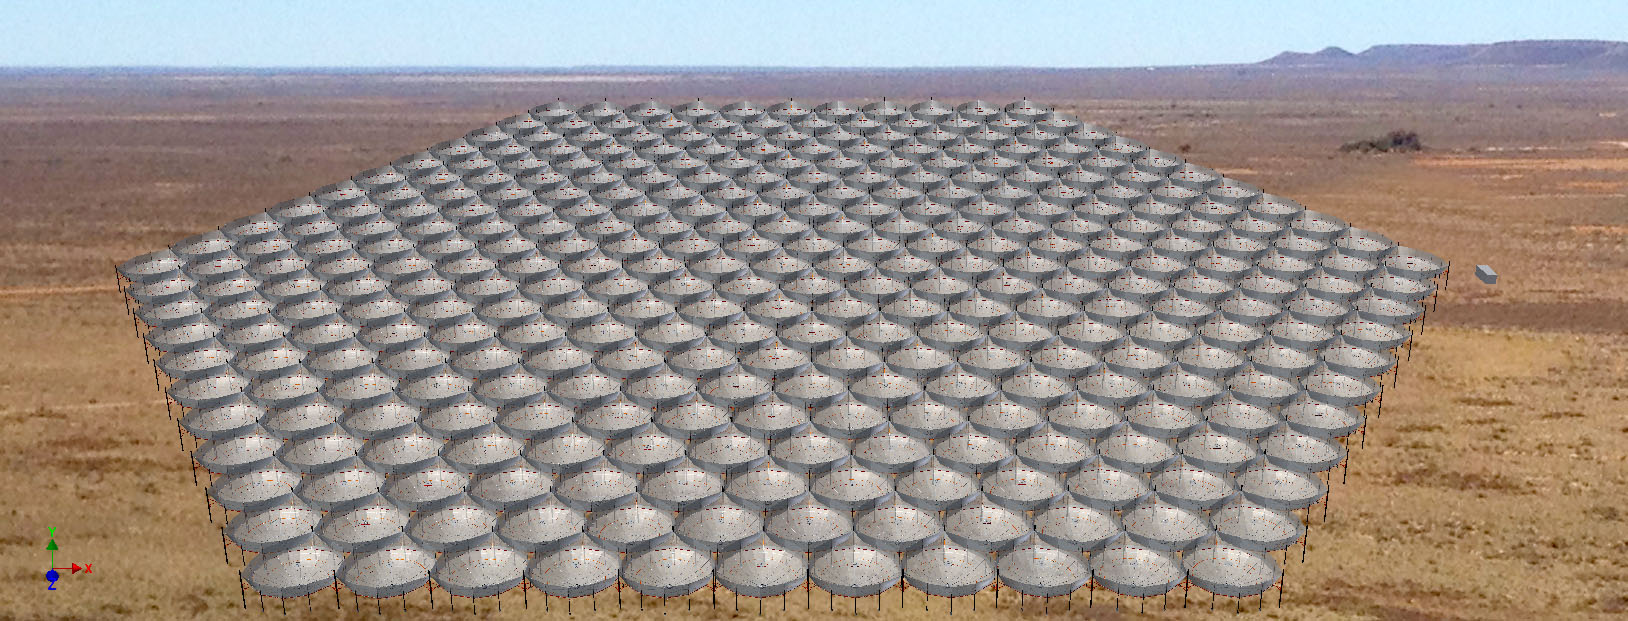
\includegraphics[width=6in]{plots/hera331perspect2.jpg}
\caption{\small
The proposed array of 331 14~m-diameter zenith-pointing dishes in the Karoo Radio Astronomy Reserve
in the Northern Cape of South Africa.
}\label{fig:hera_array} \end{figure}

% Parsons, Carilli
% A statement of which of the four categories of MSIP is most appropriate
%for this proposal as the first sentence (see section II. Program Description).
%A. We propose HERA: next step in reionization roadmap
%B. Fulfill NWNH high-priority goals
%C. New understanding/techniques => faster, better, cheaper
%D. Brief summary of timeline: science along the way, major results before end-decade

\vspace{-0.4in}
\section{Overview of this Proposal} % 1 page ~ project summary? 

% XXX
% I would really start out saying that this is a proposal to detect the EOR 21 cm
% at high enough significance to exclude models based on scale and redshift
% dependence of the power spectrum, plus map the brightest features.  The array
% itself is a consequence, not the driver, of the proposal.

The Hydrogen Epoch of Reionization Arrays (HERA) roadmap is a staged
plan for using the unique properties of the 21~cm line from neutral
hydrogen to probe our cosmic dawn, from the birth of the first 
stars and black holes, through the full reionization of the primordial
intergalactic medium (IGM). 
During these epochs, roughly 0.3--1~Gyr after the Big Bang, the
first stars and black holes heat and reionize the neutral
IGM that pervades the Universe following cosmic
recombination. Direct observation of the large scale structure of the primordial
IGM, and its evolution with time, via the \HI 21~cm line, will
have a profound impact on our understanding of the birth of the first
galaxies and black holes, their influence on the surrounding gas,
and cosmology. 

HERA was ranked the ``{\it top priority in the Radio, Millimeter, and
Sub-millimeter category of recommended new facilities for mid-scale
funding}" as part of the {\it New Worlds, New Horizons of Astronomy
and Astrophysics} decadal survey (\citealt{astro2010}; hereafter
NWNH).  The HERA roadmap initially envisioned a series of radio
interferometers constructed throughout the decade. Phase I of this roadmap
incorporated existing instruments --- the Donald C. Backer Precision Array to Probe the Epoch of
Reionization (PAPER) and the Murchison Widefield Array (MWA) ---
aimed at characterizing foregrounds and laying the
groundwork for a statistical detection of the HI 21~cm signal through
the power spectrum.  A second-generation HERA instrument would measure
the evolution of the power spectrum to reveal details of the astrophysics
involved in the birth and evolution of galaxies 
in the early Universe. A third-generation instrument would
directly image structures throughout reionization.

With a fraction of the funding recommended for HERA Phase I
in NWNH, the MWA and PAPER projects have made
major strides in developing techniques to disentangle
the reionization signal from the strong radio continuum foreground
emission.  These techniques, which are based on a new
understanding of the interplay of foreground and instrumental systematics
in the context of a three-dimensional cosmological intensity-mapping experiment,
have yielded a critical breakthrough.  As discussed below, {\bf we are now able to remove 
foregrounds to the limits of our sensitivity with these instruments},
and this is culminating in the first physically meaningful upper limits
on the power spectrum of 21~cm emission from reionization \citep{parsons_et_al2013}. PAPER
and MWA are now performing deep science observations, with the potential to 
obtain a few sigma?? detection of the HI 21cm signal within two years. 

% last sentence above could go - cc
% Carilli: I think the paragraph below is a bit repeditive. 
% In the interest of length, I have commented out and revised below

%Current generation 21~cm reionization experiments (LOFAR, MWA, PAPER) 
%are fully constructed and have been engaged in observations
%that will soon reach the sensitivity limits of these instruments.  Meanwhile,
%the principles that have yielded this breakthrough in foreground removal
%have given us new insight into how
%21~cm reionization experiments should be designed.  
%Based on these insights, we have developed a new 14~m diameter antenna element 
%that is optimized both for
%sensitivity and for minimizing foreground systematics.  
%Arranging these elements in a compact hexagonal grid yields an array that
%facilitates calibration, leverages proven foreground removal techniques, and is scalable
%to large collecting areas.

Building from lessons learned from MWA and PAPER, we have developed a new 14~m diameter antenna element 
that is optimized both for sensitivity and for minimizing foreground systematics.  
Arranging these elements in a compact hexagonal grid yields an array that
facilitates calibration, leverages proven foreground removal techniques, and is amenable 
to multiple approaches to reionization studies. We are now ready to build the instrument
that delivers HERA-II science at a cost that is substantially below what was originally envisioned in NWNH.
The proposed HERA-331 will have close to two orders of magnitude better
sensitivity than PAPER and MWA, and a wider frequency range of 50MHz to 225MHz. 
Construction will proceed in two stages, allowing for technical improvements, and delivering key science
throughout: 

\begin{itemize}[noitemsep,nolistsep]

\item HERA~127: A 127 element hexagonal array will be deployed by 
the end of the second year of this proposal. HERA-127 will measure the rise and fall of the 
21~cm reionization power spectrum from $z = 7$ to 12. HERA-127 will provide tight constrains on 
the timing and duration of reionization, and push to epochs that are difficult or impossible to 
probe with other techniques.

\item HERA~331: A 331 element hexagonal array will be deployed by the end of the third year. HERA-331 
will measure fluctuations in the 21~cm
signal over a variety of spatial
scales to determine the nature and distribution of the first galaxies
that dominate cosmic reionization. HERA~331 will also extend precision
power-spectrum observations back to the end of the 'Dark Ages' ($z \sim 20$), 
when the first stars and black holes warm the primordial IGM. In its final stages, 
HERA may be capable of imaging the largest structures in the primordial
IGM --- a task previously only considered for third-generation
instruments. 

% ARP: these designs already said below
%Ultimately, HERA-331 will have the sensitivity to
%image directly the largest scale structures in the IGM during reionization.
\end{itemize}

% XXX as above, emphasize the proposal is for the 21cm science; array is a consequence
This proposal is intended to be a self-contained package
supporting the core activities required for delivering HERA-II science,
including telescope development, construction, observing, data analysis,
and scientific products for each stage of the project.  As described
in the Project Management Plan, this approach minimizes
risks associated with external funding contingencies, but leaves room for
collaborators to leverage outside resources for augmenting the science
output of HERA in meaningful ways.

% XXX document map here?

%  ___     _                 
% / __| __(_)___ _ _  __ ___ 
% \__ \/ _| / -_) ' \/ _/ -_)
% |___/\__|_\___|_||_\__\___|


% Science currently at 5.5 pages.  

\compress
\section{Scientific Justification and Intellectual Merit} %total = 8 pages

%\subsection{Introduction}    % 1 page + 1 fig = simulated Tb cube + PS evolution
% Furlanetto, Carilli

%i.physical concepts: reionization and dark ages
%ii. Current knowledge: various constrai	nts, 1st galaxy studies...
%iii. Important role of 21~cm studies highlighted in NWNH
%a. Typical ideal sim results: T_B vs. z 'cube' and corresponding power spectrum evolution (Fig)
%b. introduce some of the important parameters/processes explored: when? how? bubble scale? sources? inside out? [much of this could be left for below?)
%c. reemphasize that current knowledge is nil, yet demand is high
%d. emphasize unique (only?) probe of dark ages

The {\it cosmic dawn}, the period beginning with the birth of the first stars and culminating with the full
reionization of the IGM some 500 Myrs later, represents one of the last unexplored phases in 
the cosmic history. This period is rich in both astrophysical and cosmological phenomena. 
The characteristics of the IGM depend on the cosmic density field, the first galaxies (e.g., their typical masses and clustering), their constituents (e.g., exotic Pop. III 
stars, more normal stars, stellar remnants, or supermassive black holes), their ultraviolet luminosities (which affect  IGM ionization), the efficiency and abundance of X-ray sources (which affect IGM temperature), and 
cosmological effects like the relative velocity of baryons and dark matter. 
Exploring these early structures, and their interplay with their environment was one of the top three ``{\it priority science objectives chosen by 
the [NWNH] survey committee for the decade 2012-2021.}

% I have revised below, in light of Fan's comment that we need to highlight how 21cm fits into the broader 
% picture of study of F(HI) and first galaxies

Study of the evolution of the neutral IGM and reionization has historically been a high priority in astronomy, and is a motivator for future large telescopes.  Recent measurements from the {\it Hubble Space Telescope} have pinned down the bright end of the galaxy luminosity function 
at $z \la 8$ \citep{bouwens_et_al2010, schenker_et_al2013} and have detected a few sources at even greater 
distances \citep{ellis_et_al2013, oesch_et_al2013}. Still, a complete census of the galaxies required for
reionization requires deep observations with eg. JWST and ALMA, to reveal the fainter end of the luminosity function. 
In parallel, a number of indirect techniques have been used to constrain the evolution of the neutral fraction
with redshift, although predominantly at the end of reionization. Figure~\ref{fig:x_i_vs_z} summarizes 
these results, including: 

\begin{itemize}[noitemsep,nolistsep]

\item Observations of resonant scattering of Ly$\alpha$ by the neutral IGM toward
distant quasars (the 'Gunn-Peterson' effect) \citep{fan_et_al2006}.

\item The demographics of Ly$\alpha$ emitting  galaxies \citep{schenker_et_al2012, treu_et_al2013,Faisst_et_al2014}.

\item The Ly$\alpha$ absorption profile toward the most distant quasar ($z = 7.1$) \citep{bolton_et_al2011}.

\item Measurements of the optical depth to reionization based on CMB temperature fluctuations \citep{planck_et_al2013} and large scale polarization anisotropies \citep{page_et_al2007}.

\item Secondary temperature fluctuations generated by the kinetic Sunyaev-Zel'dovich effect \citep{zahn_et_al2012_trunc, mesinger_et_al2012}. 

\end{itemize}

Results from these observations suggest that the IGM may have been substantially neutral even at $z \sim 7$--8 (as high as $F_{HI} \sim 0.5$), with a tail of finite ionization ($\sim 0.1$) extending to high 
redshift ($z \sim 15$).  Unfortunately, these methods (while extremely informative), have limited reach:
(i) Gunn-Peterson
and related effects probe only the tail-end of reionization, (ii) strong assumptions 
are required about the stellar populations, the escape fraction of UV photons from the galaxies, and the
clumping of the IGM, and (ii) the CMB provides only an integral measure of the ionized IGM back to recombination. 
Moreover, many of these indirect observations are in tension with one another, underscoring both the difficulty in 
their interpretation and the complexity of the reionization process.

The 21~cm ``spin-flip" transition of  neutral hydrogen has been recognized as potentially the most powerful probe 
of cosmic reionization and  the dark ages \citep{morales_wyithe2010, furlanetto_et_al2006}, as emphasized in NWNH: 
``{\it 
%SF: Is this quote from the RMS panel?  If so, does it appear in the final report?
The panel concluded that  to explore the discovery area of the epoch of reionization, it is most important to 
develop new capabilities to observe redshifted 21~cm \HI emission, building on the legacy of current projects and 
increasing sensitivity and spatial resolution to characterize the topology of the gas at reionization.}"  Because 
our Universe is almost entirely neutral before reionization, the HI 21~cm line provides a direct method to image 
the evolution of the primordial IGM, opening a unique window into the complex astrophysical interplay between the 
first luminous structures and their surroundings. Moreover, because of the cosmological redshift, we can associate 
the signal at each observed frequency with a particular emission time (or distance) and reconstruct a complete 
three-dimensional picture of the time evolution of large scale structure during this `last frontier' in 
observational cosmology. 
%SF: Personally I feel like the following is an exaggeration that could rub some people the wrong way!
%The direct observation of the primordial IGM via the HI 21~cm line would be an achievement comparable in importance 
%to the detection of anisotropies in the CMB.

%\begin{figure}[t]\centering
%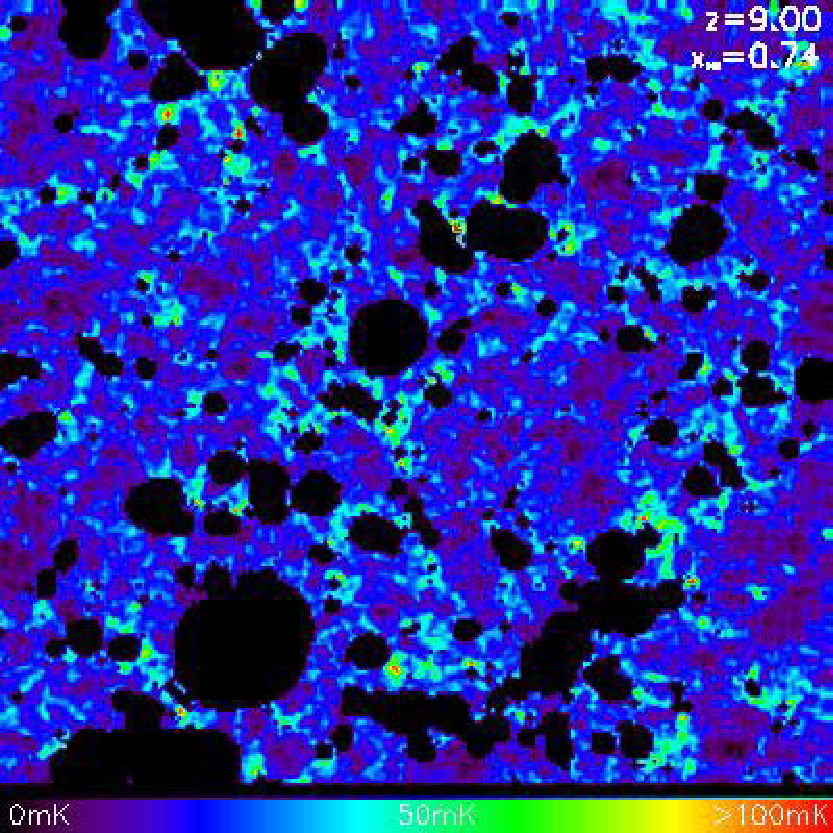
\includegraphics[width=0.23\textwidth]{plots/Pspec/z9sim.pdf}
%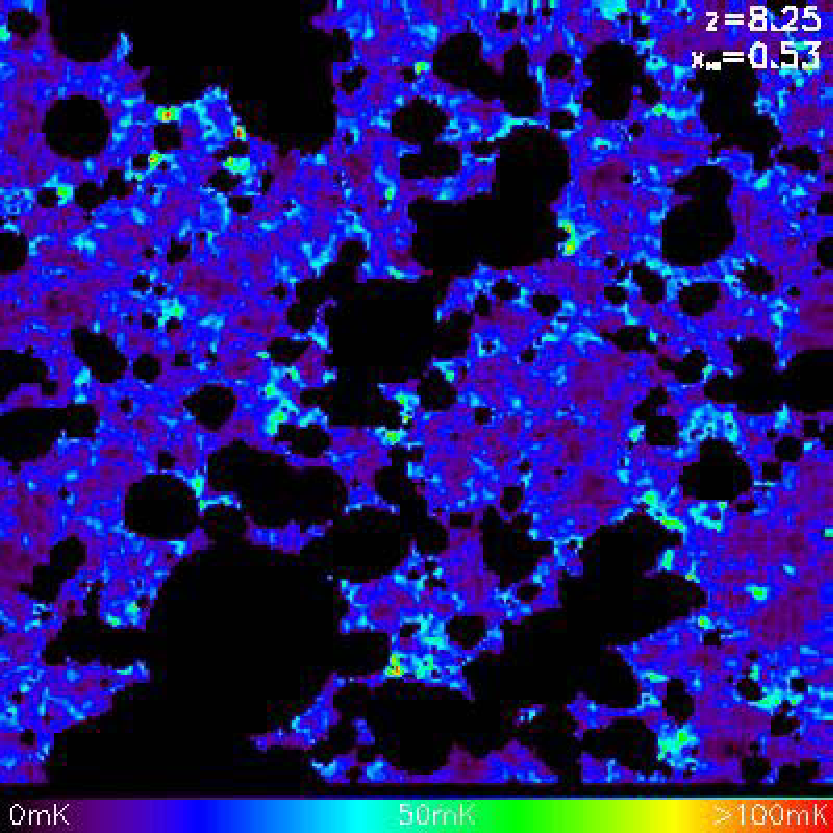
\includegraphics[width=0.23\textwidth]{plots/Pspec/z8sim.pdf}
%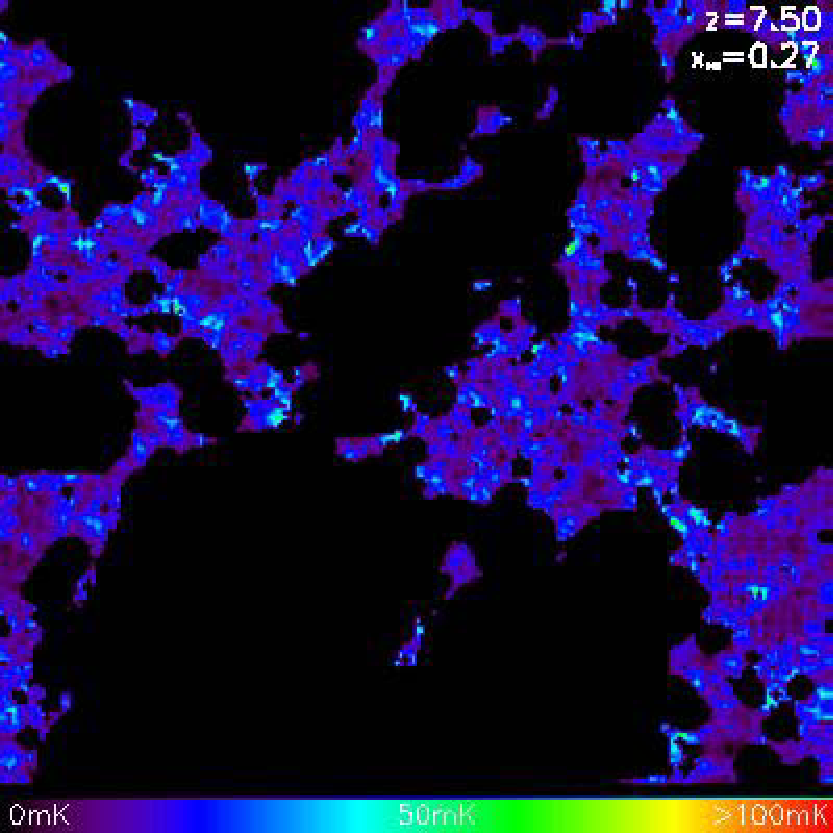
\includegraphics[width=0.23\textwidth]{plots/Pspec/z75sim.pdf}
%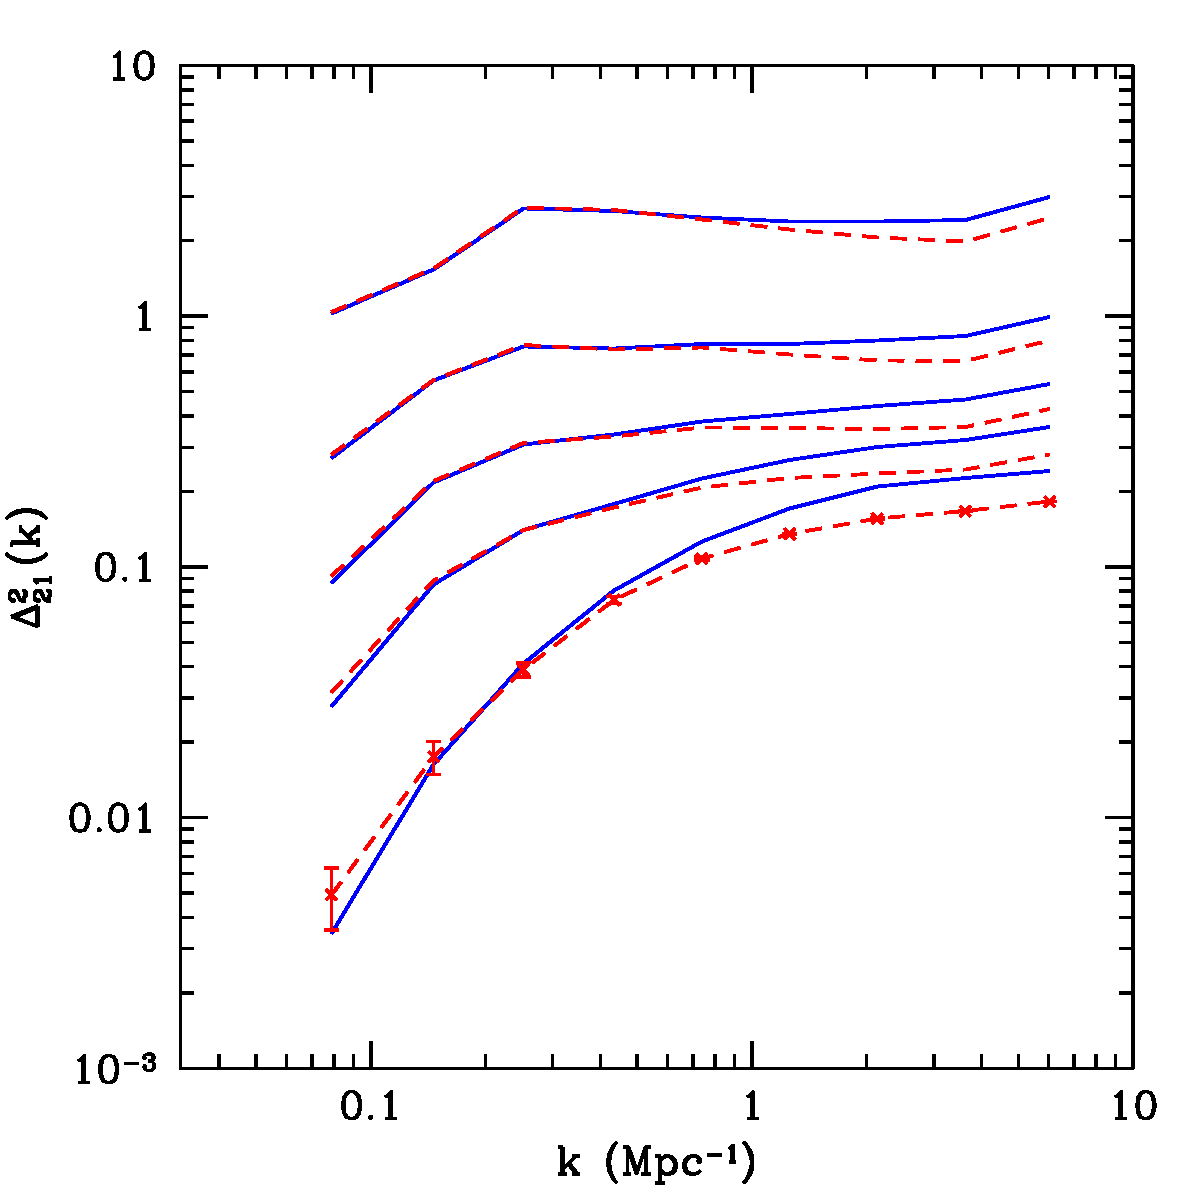
\includegraphics[width=0.23\textwidth]{plots/Pspec/pspecEvolve.pdf}
%\caption{\small 
%First three panels from left: simulated $21\,\textrm{cm}$ brightness temperature distributions at $z=9$, $8$, and $7.5$.  Rightmost panel: Evolution of the $21\,\textrm{cm}$ power spectrum from $z=9.25$ to $z=7$.  HERA will characterize the power spectrum in detail (Section \ref{sec:detectPspec}) as well as provide images of the ionized bubbles (Section \ref{sec:imaging_HI}).
%}\label{fig:EoRsims} \end{figure}

\begin{figure}[t]\centering
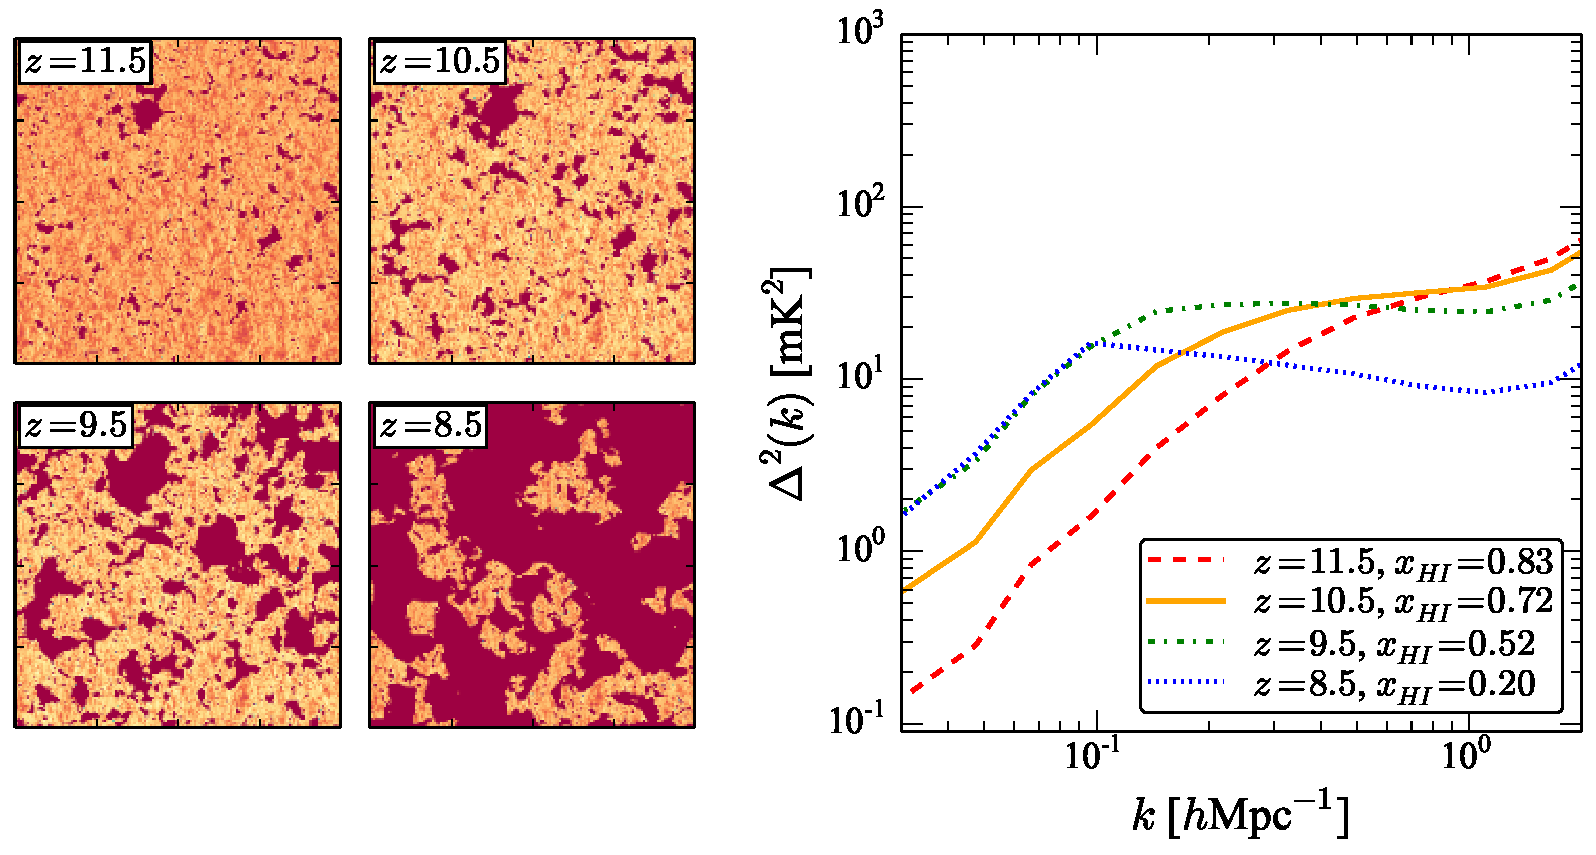
\includegraphics[height=2.5in]{plots/cubes/cubesAndPspecs.pdf}
\caption{\small 
Left: Simulated 21~cm brightness temperature distributions spanning $\sim 280 \times 280\,h^{-1}\textrm{Mpc}$.
at $z=11.5$, $10.5$, $9.5$, and $8.5$.
Right: Corresponding evolution of the 21~cm power spectrum.  HERA
will characterize the power spectrum in detail (\S\ref{sec:detectPspec}), as well as
provide images of the ionized bubbles (\S\ref{sec:imaging_HI}).
}\label{fig:EoRsims} \end{figure}

Decades of effort has gone into modeling the complex astrophysics of reionization
(e.g. \citealt{shapiro_giroux1987, haiman_loeb1997, furlanetto_et_al2004, santos_et_al2010}). Figure \ref{fig:EoRsims} shows a 
simulation of the expected evolution of the HI 21~cm signal during reionization \citep{mesinger_furlanetto2007}. Fluctuations in the signal initially 
rise above those expected from the cosmic density field due to the growth of ionized bubbles on a characteristic 
scale of a few to 10~arcmin. This scale is set by the clustering of early galaxy formation, as well as by 
propagation effects through the IGM. The signal then declines as the IGM becomes fully ionized.  These theoretical 
models of the reionization process are sophisticated and appear to be well-understood, {\it but they are not 
predictive tools.} Instead, they provide a mapping between the largely unknown galaxy populations and observables 
like the 21~cm transition. As such, the key questions about the cosmic dawn era remain poorly understood.  When 
did reionization occur, and over what timescale?  What objects dominated the radiation field?  How were the 
objects distributed?  What were the most important feedback mechanisms in the transition from the first stars to
first galaxies, and how did they affect these populations?  {\it HERA provides the key measurements that are needed 
to advance our understanding of early galaxy formation and cosmic reionization.}


%Figures: F(HI) vs z;  HI Tb cube + PS evolution


\compress
\subsection{Reionization and Dark Ages Science} % 4 pages total examples using hera 331, plus a number of figures

\begin{figure}[t]\centering
%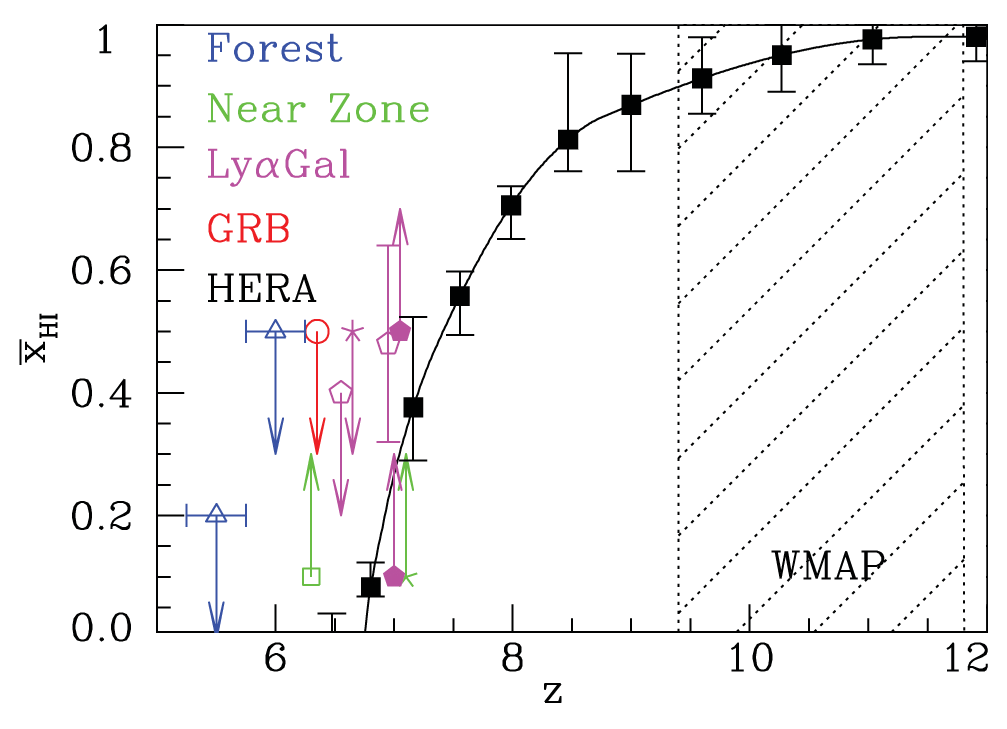
\includegraphics[height=2.25in]{plots/constraints_crop.pdf} 
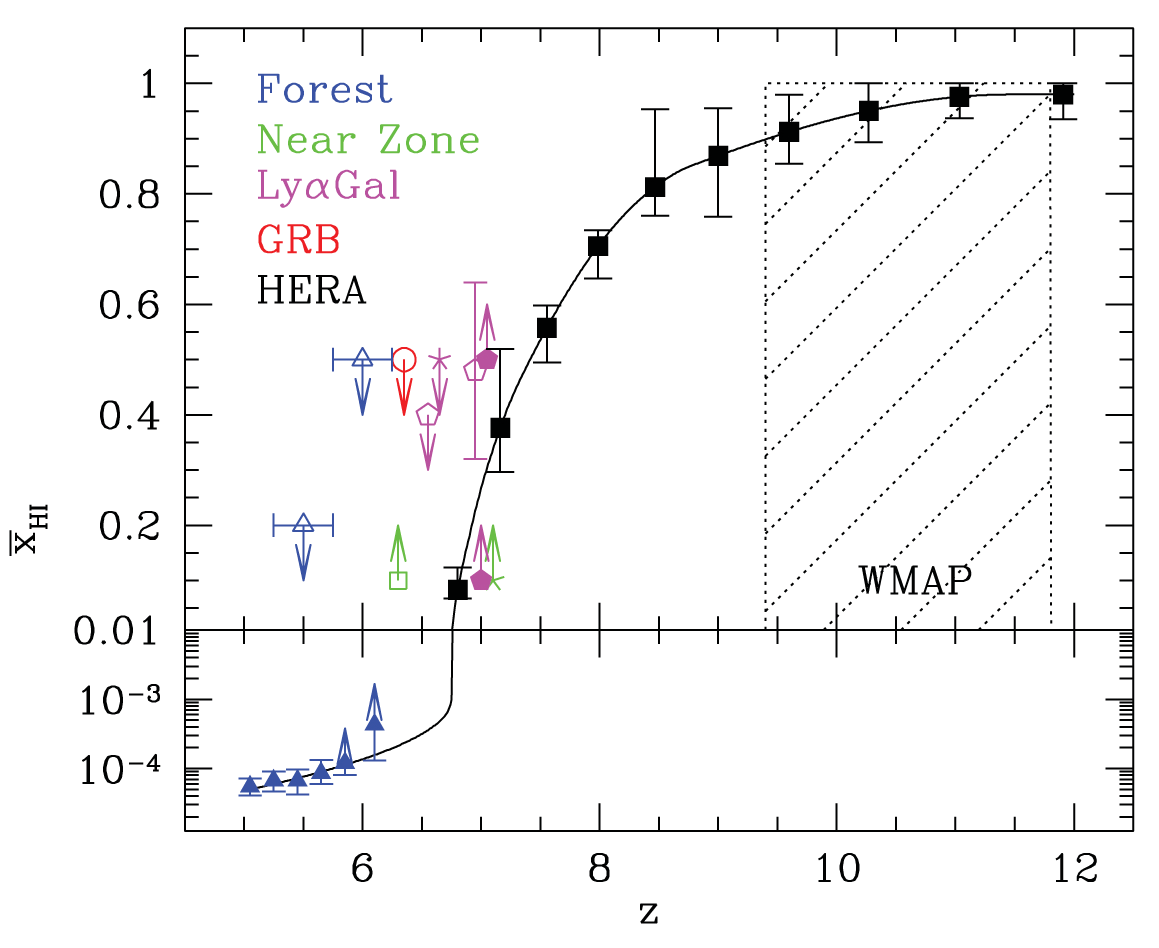
\includegraphics[height=2.25in]{plots/constraints.pdf}
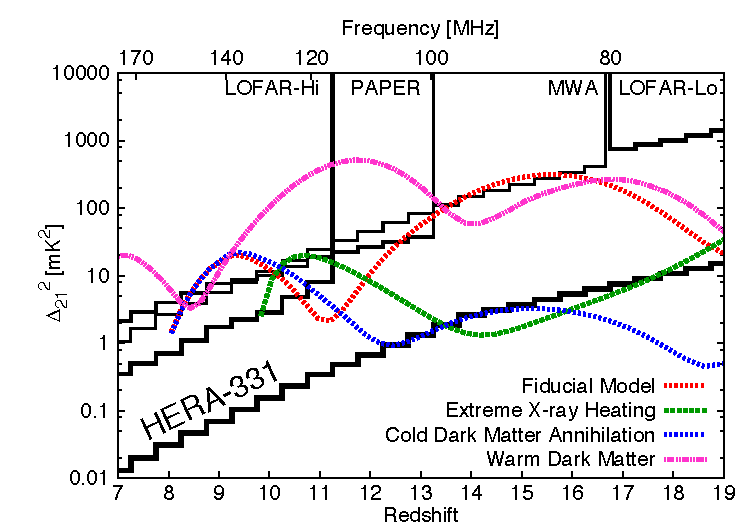
\includegraphics[height=2.25in]{plots/Xray/HERA_II_compare_kp1_whoriz_20pt.pdf} 
\caption{\small 
Left: 
Existing
constraints on neutral fraction ($\xHI$) versus redshift (adapted from \citealt{robertson_2013}), along with 
prediected HERA constraints (black markers)
%assuming that $\xHI$ decreases versus redshift
for a fiducial
reionization history (black line).
At $z>8$,
21~cm emission may be the only precise probe of $\xHI$.
Right: At lower frequencies, HERA probes
pre-reionization physics at the end of the Dark Ages. Plotted are power spectrum amplitudes (at $k =
0.15h$~Mpc$^{-1}$) for various IGM heating models \citep{mesinger_et_al2013},
with predicted sensitivities.
}\label{fig:x_i_vs_z} \end{figure}

As a high-sensitivity instrument with broad frequency coverage, HERA can
paint an uninterrupted picture through reionization, back to the end of 
the Dark Ages. This capability leverages the coupling of
21~cm emission to the properties of the first galaxies that
are inaccessible through other means,  and will be transformative for
studying the imprint of the very first galaxies in the Ly-$\alpha$ and X-ray backgrounds.  
Figure~\ref{fig:x_i_vs_z} illustrates how HERA will
determine the ionization history of our universe much more precisely,
and at higher neutral fractions (wider redshift range), than is possible with other existing techniques.  
These measurements can
be used to move beyond characterizing the timing and duration of reionization to
explore which galaxies dominate the integrated UV luminosity density, what the escape fraction
of UV photons is in early galaxies, and how feedback from early star formation affects low-mass galaxies and 
the integrated  global ionization profile versus redshift (see \S\ref{sec:ParamEst} regarding parameter estimation). 
At earlier epochs ($z \sim 15$ to 20), the sensitivity of the 21~cm line 
to the IGM temperature provides a unique probe of processes that warm the neutral IGM at the
end of the dark ages.  HERA will have the low frequency coverage and
sensitivity to study these earliest phases of star and black hole formation -- an epoch that may be otherwise
untestable using other techniques.

\compress
\subsubsection{Detecting and characterizing the power spectrum}
\label{sec:detectPspec}
